\begin{center}
  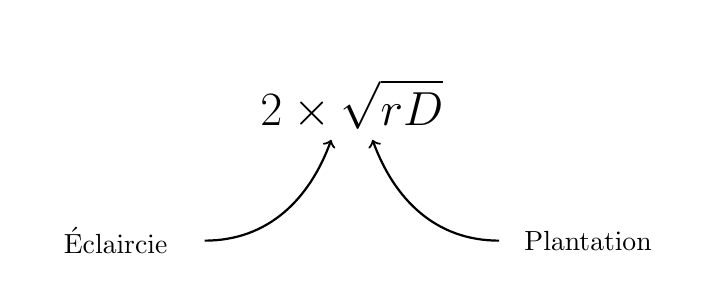
\begin{tikzpicture}[thick,every text node part/.style={align=center}]

    % --------------------------------------------------------- %
    % ------------- principal node (Formula)
    % --------------------------------------------------------- %
    \node[text width=6cm,minimum height=1cm,minimum width=3cm] (formule) at (10,10) {\LARGE{$$2 \times \sqrt{rD}$$}};

    % --------------------------------------------------------- %
    % ------------ Effect of forst management
    % --------------------------------------------------------- %
    \node[text width=2cm] (ecl) at (7,8) {Éclaircie};
    \draw [->] (ecl) edge [in=250, out=0] (formule);

    \node[text width=2cm] (plant) at (13,8) {Plantation};
    \draw [->] (plant) edge [in=290, out=180] (formule);

  \end{tikzpicture}
\end{center}
